\documentclass{VUMIFPSbakalaurinis}
\usepackage{algorithmicx}
\usepackage{algorithm}
\usepackage{algpseudocode}
\usepackage{amsfonts}
\usepackage{amsmath}
\usepackage{bm}
\usepackage{caption}
\usepackage{color}
\usepackage{float}
\usepackage{graphicx}
\usepackage{listings}
\usepackage{subfig}
\usepackage{wrapfig}
%
%
%% Mano pridėti paketai
\usepackage{longtable}
\usepackage{enumitem}
\usepackage[none]{hyphenat}
%\usepackage{listings}
%\usepackage{xcolor}
\usepackage{pdflscape}
\usepackage{seqsplit} % for \seqsplit macro
%\usepackage{footmisc}

\usepackage{color}
\definecolor{lightgray}{rgb}{.9,.9,.9}
\definecolor{darkgray}{rgb}{.4,.4,.4}
\definecolor{purple}{rgb}{0.65, 0.12, 0.82}

\lstdefinelanguage{JavaScript}{
  keywords={typeof, new, true, false, catch, function, return, null, catch, switch, var, if, in, while, do, else, case, break, address, uint256, public, event, constructor, uint, contract, for},
  keywordstyle=\color{blue}\bfseries,
  ndkeywords={class, export, boolean, throw, implements, import, this, is},
  ndkeywordstyle=\color{darkgray}\bfseries,
  identifierstyle=\color{black},
  sensitive=false,
  comment=[l]{//},
  morecomment=[s]{/*}{*/},
  commentstyle=\color{purple}\ttfamily,
  stringstyle=\color{red}\ttfamily,
  morestring=[b]',
  morestring=[b]"
}

\lstset{
   language=JavaScript,
   backgroundcolor=\color{lightgray},
   extendedchars=true,
   basicstyle=\footnotesize\ttfamily,
   showstringspaces=false,
   showspaces=false,
   numbers=left,
   numberstyle=\footnotesize,
   numbersep=9pt,
   tabsize=2,
   breaklines=true,
   showtabs=false,
   captionpos=b
}

%neperklti į kitą eilutę
\hyphenation{PLSE}
\hyphenation{ICO}
\hyphenation{FORM}
\hyphenation{FODA}
\hyphenation{blockchain}
\hyphenation{TokenMarket}
\hyphenation{OpenZeppelin}
\hyphenation{STO}


 %Titulinio aprašas
\university{Vilniaus universitetas}
\faculty{Informatikos institutas}
\department{Programų sistemų katedra}
\papertype{Bakalauro baigiamasis darbas}
\title{Pakartotinis kodo panaudojimas pirminio kriptovaliutų platinimo išmaniuosiuose kontraktuose}
\titleineng{Code Reuse in Initial Coin Offering Smart Contracts}
\author{Agnė Mačiukaitė}
\supervisor{lekt. Gediminas Rimša}
\reviewer{partn. doc. Vaidas Jusevičius}
\date{Vilnius – \the\year}
% Nustatymai
% \setmainfont{Palemonas}   % Pakeisti teksto šriftą į Palemonas (turi būti įdiegtas sistemoje)
\bibliography{library}
%
\begin{document}
\maketitle

%% Padėkų skyrius
% \sectionnonumnocontent{}
% \vspace{7cm}
% \begin{center}
%     Padėkos asmenims ir/ar organizacijoms
% \end{center}
\sectionnonumnocontent{Santrauka}

%Kodo pernaudojamumas svarbus norint užtikrinti sistemos kūrimo efektyvumą. Tarp 2014 metų sausio ir 2018 metų birželio pirmininis kriptovaliutų platinimas (angl. initial coin offering, toliau ICO) surinko daugiau nei 18 milijardų dolerių. Dauguma kuria ICO išmaniuosius kontraktus ir talpina juos Ethereum blokų grandinėje. Taip per trumpą laiką buvo sukurta daug panašių išmaniųjų kontraktų. Pernaudojamumo problema bandoma spręsti Ethereum bibliotekomis, tačiau jos ne visada padengia visą savybių aibę. Savybių modeliavimas yra būdas valdyti savybes produktų linijoje. Jis yra efektyvus ir intuitivus būdas išreikšti savybių paplitimą ir kintamumą srityje. Savybių pernaudojamumo metodas praplečia savybių modeliavimą ir nusako, kaip turint savybių modelį, sukurti srities architektūra ir komponentus.


Per neilgą laikotarpį Ethereum blokų grandinėje buvo sukurta daug pirminio kriptovaliutų platinimo išmaniųjų kontraktų, kurių kodas kartojasi. Kodo pakartojamumo problemą bandoma spręsti bibliotekomis. Šiame darbe kodo pakartojamumo problema tiriama pasitelkiant savybių modeliavimą. Pirmiausia interneto skaitytuvu buvo surinkti 161 pirminiam kriptovaliutų platinimui skirti išmanieji kontraktai, patalpinti Ethereum blokų grandinėje, iš kurių 40 buvo panaudoti sudarant savybių modelį. Tuomet, darbe sudaromi savybių modeliai atspindintys populiariausias Ethereum bibliotekas OpenZeppelin ir TokenMarket. Atlikus savybių modelių palyginimą tarp blokų grandinėje esančių išmaniųjų kontraktų ir bibliotekų, nustatyta, kad bibliotekos nepilnai padengia reikalingą savybių aibę. OpenZeppelin bibliotekai trūksta 9 savybių bei turi vieną perteklinę, TokenMarket bibliotekai trūksta trijų savybių. Tam, kad būtų padidinamas kodo pakartojamumas, nuspręsta pasiūlyti pakeitimus TokenMarket bibliotekai.

\raktiniaizodziai{pirminis kriptovaliutų platinimas, blokų grandinė, išmanieji kontraktai, savybių modeliavimas, savybių pernaudojimo metodas}

\sectionnonumnocontent{Summary}

% KS edited

A lot of initial coin offering smart contracts were created in a short period. However, the code of those smart contracts often repeats across multiple smart contracts. Some Ethereum smart contract libraries are trying to solve this code reusability problem. In this thesis, the problem of repetitive code is being looked at from the perspective of feature modelling. Firstly, using a web crawler, 161 initial coin offering smart contracts were collected and 40 of them have been used composing a feature model. Then, feature models were composed for the most popular Ethereum libraries: OpenZeppelin and TokenMarket. After performing the comparison between the smart contracts from Ethereum blockchain and libraries, it was found that the Ethereum libraries do not exhibit all the required features. Namely, OpenZeppelin library is missing 9 features and has one redundant feature. Whereas, TokenMarket library is missing 3 features. As a contribution to code reuse improvement, changes to TokenMarket library were suggested.

% In this thesis, feature models of Ethereum initial coin offering smart contracts are investigated. .   In this thesis features are used to define repetitive code in the initial coin offering smart contracts. Three types of initial coin offering smart contracts were studied: smart contracts which are published on Ethereum blockchain, smart contracts from OpenZeppelin and TokenMarket libraries. In this thesis, features of these initial coin offering smart contracts, creates features models and compares the created feature models are studied. It was found that Ethereum libraries do not have all the required features. OpenZeppelin library is missing 9 features and has one redundant feature. TokenMarket library is missing 3 features. Taking it to account, changes to TokenMarket library were suggested.

\keywords{initial coin offering, blockchain, smart contracts, feature-oriented domain analysis, feature-oriented reuse method}

\tableofcontents

\sectionnonum{Įvadas}



Kodo pernaudojimas suteikia galimybę naudoti programas keliuose projektuose. Tai yra svarbi strategija kodui, norint padidinti sistemos kūrimo efektyvumą ir kokybę. Taikant pernaudojamumą programuotojai naudojasi jau įgyvendintu kodu, kurį keičia taip, kad jis atitiktų naujo projekto reikalavimus \cite {Ravichandran2003}. Viena iš būtinų sąlygų, kuriant pernaudojamą kodą yra supratimas skirtingų kontekstų, kuriuose pernaudojamas kodas galėtų būti naudojamas ir kaip būtų valdomas jo pernaudojamumas. Tai padeda programuotojams nuspręsti ar kodas atitinka reikalavimus ir ar gali būti kuriamas, jei taip, tai ką reikia parametrizuoti ir kaip struktūrizuoti kodą, kad vėliau būtų galima jį pritaikyti skirtingiems kontekstams \cite{Kang1990}.


Pirminio kriptovaliutos platinimo (angl. initial coin offering, toliau ICO) metu įmonė parduoda specializuotus kripto-žetonus žadėdami, kad žetonai veiks kaip mainų priemonė atsiskaitant už paslaugas įmonės platformoje. Žetonų pardavimas kuria kapitalą pradiniam įmonės platformos kūrimui, nors nėra įsipareigojimo dėl būsimos paslaugos kainos (žetonais ar kitaip) \cite{Catalini2018}.  Tarp 2014 m. sausio ir 2018 m. birželio, ICO surinko daugiau nei 18 milijardų dolerių. Lėšų surinkimas ICO būdu pritraukė verslininkų, investuotojų ir reguliavimo įstaigų dėmesį. Dauguma ICO kuria išmaniuosius kontraktus (automatizuotą programinę įrangą) ir juos talpina Ethereum blokų grandinėje \cite{Howell2018}.

Neseniai iškilęs ICO populiarumas yra paveiktas Bitcoin kriptovaliutos ir Ethereum kriptovaliutos su papildoma programavimo galimybe \cite{Catalini2018}. Ethereum ir Bitcoin šiuo metu dvi populiariausios blokų grandinės (angl. blockchain, toliau blockchain) \cite{Luu}. Bitcoin - skaitmeniniai pinigai, kurių pavedimai vyksta internete naudojantis decentralizuota vieša duomenų baze - blockchain \cite{Swan2015}. Ethereum be savo kriptovaliutos turi ir kitą svarbų funkcionalumą - išmaniuosius kontraktus - Turing pilną (angl. complete) programą, kuri leidžia rašyti decentralizuotas aplikacijas \cite{Buterin2014}. Solidity - populiariausia kalba, naudojama rašyti išmaniesiems kontraktams \cite{Dannen}.

Problema - per trumpą laiką buvo sukurta daug panašių išmaniųjų kontraktų, kurie dažnai kuriami kopijuojant jau esamus ICO išmaniuosius kontraktus bei pridedant reikiamus pakeitimus. Taip sukurta didelė aibė ICO išmaniųjų kontraktų, kurių kodas yra labai panašus arba kartojasi. Pernaudojamumo problemą spręsti bandoma Ethereum išmaniųjų kontraktų bibliotekomis, tačiau jos ne visada padengia visą ICO išmaniųjų kontraktų savybių aibę.

Produktų linijos programų inžinerija (angl. product line software engineering, toliau PLSE) naudojama įmonėse pakartojamumui susijusiuose aplikacijose numatyti. Kodas yra kartojamas skirtinguose produktuose tam, kad būtų užtikrintas jo pernaudojamumas. PLSE suteikia bendrą architektūrą ir pernaudojamą kodą aplikacijos kūrėjams \cite{Svahnberg}. PLSE kūrimas susideda iš savybių išskyrimo ir jų įgyvendinimo produkte. Gerai išskirtos produkto savybės padeda sukurti lengvai pernaudojamą programą. Savybės turi būti atrinktos atsižvelgiant į jų paplitimą bei kintamumą dalykinėje srityje \cite{Lee2015}.

Savybių modeliavimas yra pagrindinis metodas atrinkti bei valdyti bendrąsias ir kintamas savybes produktų linijoje. Programų inžinerijos šeimos gyvavimo pradžioje savybių modelis padeda išskirti pagrindines savybes, kurios gelbsti kuriant naują rinką ar  norint išlikti jau esamoje. Taip pat savybių modelis leidžia išskirti rizikingas savybes, nuspėti visos programos ar atskirų savybių kainą. Vėliau savybių modeliavimas padeda išskirti variacijos taškus programos architektūroje \cite{Czarnecki2004}. Savybių modeliavimas yra populiariausias metodas PLSE kūrime nuo pat pirmojo jo pristatymo \cite{Kang1990}. Savybės yra pakankamai abstraktus konceptas, padedantis efektyviai bendrauti suinteresuotoms šalims. Savybių modeliavimas yra intuityvus ir efektyvus būdas, žmonėms išreikšti savybių paplitimą ir kintamumą programos inžinerijos šeimoje \cite{Kang2013}.

Savybių pernaudojimo metodas (angl. feature-oriented reuse method, toliau - FORM) praplečia savybių modeliavimą bei nusako, kaip remiantis savybių modeliu sukurti programos inžinerijos architektūrą ir komponentus. FORM teigia, kad savybės apibūdina galimus galutinio produkto variantus, o kodas, kuris įgyvendina savybes, turi būti sukurtas pakartotiniam panaudojimui. Savybių modelis naudojamas pagelbėti srities architektūros kūrime bei programavime naudojant srities artefaktus. Išanalizavus bendrumą naudojantis savybių analize, savybių modelis yra naudojamas sukurti architektūrą bei komponentus \cite{Kang}.

Šio darbo tikslas - patikrinti ar Ethereum bibliotekos padengia visas savybes, kurias turi ICO išmanieji kontraktai patalpinti Ethereum blockchain, bei pasiūlyti būdą ICO išmaniųjų kontraktų kodo pernaudojamumui didinti.

%Šio darbo tikslas - sukurti savybių modelį, atvaizduojančiu Ethereum blockchain patalpintų ICO išmaniųjų kontraktų savybes, remiantis juo patikrinti ar Ethereum bibliotekos padengia visas savybes, bei pasiūlyti būdą ICO išmaniųjų kontraktų kodo pernaudojamumui didinti.

Tikslui pasiekti išsikelti uždaviniai:
\begin{enumerate}[topsep=0pt,itemsep=-1ex,partopsep=1ex,parsep=1ex]
\item Išskirti savybių modelį ICO išmaniesiems kontraktams, patalpintiems Ethereum blockchain, ir jį validuoti;
\item Išskirti ICO savybių modelius OpenZeppelin ir TokenMarket bibliotekoms;
\item Palyginti savybių modelį, išskirtą iš Ethereum blockchain esančių ICO išmaniųjų kontraktų, su OpenZeppelin ir TokenMarket savybių modeliais;
\item Pasiūlyti pakeitimus vienai iš bibliotekų (tai, kuri yra labiau išvystyta), remiantis savybių modelių palyginimu.
\end{enumerate}


\section{Savybių modeliavimas} \label{modeliavimas}

Savybių modeliavime bendri ir kintami bruožai yra modeliuojami iš produkto savybių perspektyvos dalykinėje srityje. Savybės yra pagrindinis produkto skiriamasis bruožas \cite{Lee2015}. Keli tos pačios srities programų inžinerijos produktai turi daug bendrų bruožų, bet taip pat kiekvienas produktas turi ir savo išskirtinumų. Tie bruožai iš naudotojo perspektyvos yra savybės \cite{Kang1990}. Savybės yra suskirstytos į būtinas, alternatyvias ir pasirenkamas pagal bendrus ir kintamus bruožus \cite{Kang2013}. Originalus savybių modeliavimas - FODA (angl. Feature-Oriented Domain Analysis (FODA), toliau FODA) \cite{Kang1990} - paprastas modeliavimas, kuris savybes skirsto pagal „susideda iš" santykį bei pagal bendrumą ir specializaciją naudojant IR/AR (angl. AND/OR)  diagramas.

\subsection{Savybė} \label{savybe}

Skirtingi srities analizės metodai terminą savybė apibūdina šiek tiek kitaip \cite{Lee2015}. FODA \cite{Kang1990} savybę apibūdina kaip pastebimą ir skiriamą sistemos charakteristiką, kuri yra matoma įvairioms suinteresuotoms šalims.

FODA fokusuojasi į kliento perspektyvą - ties paslaugomis, kurias teikia aplikacija ir aplinka, kurioje dirbama. Savybės yra programinės įrangos atributai, kurie tiesiogiai paveikia naudotoją \cite{Kang1990}. Skirtumas tarp savybės ir konceptualios abstrakcijos (pvz.: funkcijos, objekto) yra tai, kad funkcijos ir objektai yra naudojami specifikuojant vidines programinės įrangos detales. Kitaip, funkcijos ir objektai yra konceptualios abstrakcijos, kurios yra identifikuojamos iš vidinės programinės įrangos pusės. Savybė - aiškiai matoma  pagal charakteristiką, kuri gali išskirti produktą iš kitų. Todėl savybių modeliavimas turi išskirti iš išorės matomas charakteristikas produktuose bendrumo ir kintamumo atžvilgiu, o ne apibūdinti visas produkto modeliavimo detales (pvz.: funkcinis, objektinis modeliavimas). Suprantant produkto bendras ir kintamas savybes galima sukurti pernaudojamas funkcijas ir objektus \cite{Lee2015}.

\subsection{Savybių modelis}

FODA \cite{Kang1990} autoriai apibrėžia savybių modelį, kaip modelį, kuris turi pavaizduoti standartines savybes dalykinėje srityje ir santykius tarp jų. Trumpiau - savybių modelis yra hierarchiškai išskirstytų savybių rinkinys - „susideda iš" santykių rinkinys \cite{Kang1990, Batory2005}. Santykiai tarp savybių  modelyje yra kategorizuojami į (\ref{img:fm_rules} pav.):
\begin{itemize}[topsep=0pt,itemsep=-1ex,partopsep=1ex,parsep=1ex]
\item Ir - visos vaikinės savybės turi būti pasirinktos;
\item Alternatyva - tik viena vaikinė savybė gali būti pasirinkta;
\item Ar - viena ar daugiau gali būti pasirinkta;
\item Privaloma - savybė yra privaloma;
\item Pasirenkama - savybė gali būti pasirenkama.
\end{itemize}

%\pagebreak

\begin{center}
    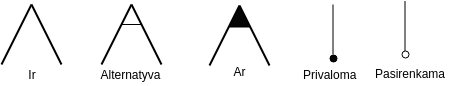
\includegraphics[scale=0.75]{img/feature_model_rules}
    \captionof{figure}{Santykių kategorijos tarp savybių \cite{Batory2005}}
    \label{img:fm_rules}

\end{center}

Savybių diagrama yra grafinė savybių modelio reprezentacija. Tai modelis - medis, kur primityvios savybės - lapai, pagrindinės - mazgai (modelio pavyzdys - \ref{img:fm_example} pav.). Būtinos savybės tarp skirtingų produktų yra modeliuojamos kaip privalomos, kai skirtingos savybės tarp jų žymimos kaip alternatyvios ar pasirenkamos (angl. optional) \cite{Batory2005}. Pagrindinės savybės atributai yra paveldimi pagal visą jos specifikaciją. Visos pasirenkamos ar alternatyvios savybės, kurios negali būti pasirinktos, kai yra bendra savybė pasirinkta turi būti pažymėtos kaip tarpusavyje nesuderinamos (angl. mutually exclusive with). Visos pasirenkamos ir alternatyvios savybės, kurios turi būti pasirinktos, kai bendra yra pasirinkta, turi būti pažymėtos kaip privalomos. Savybių modelio dokumentacija susideda iš struktūrinės diagramos hierarchiškai suskaidančios savybes identifikuojančias pasirenkamas ir alternatyvias savybes, savybių apibūdinimo ir taisyklių kompozicijos savybėms \cite{Kang1990}.

\begin{center}
    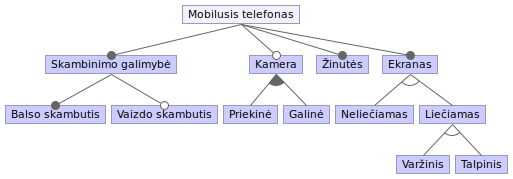
\includegraphics[scale=0.6]{img/mobile}
    \captionof{figure}{Savybių modelis mobiliajam telefonui \cite{Kang2013}}
    \label{img:fm_example}
\end{center}

Pasirenkamos ir alternatyvios savybės negali būti atrinktos savavališkai. Įprastai jos parenkamos pagal galutinio naudotojo (kliento) tikslus ar interesus \cite{Kang1990}. Reikalavimai ir funkcijos yra apibūdinami kaip savybės, kadangi jos yra aiškiai atpažįstamos abstrakcijos (plačiau \ref{savybe}. Savybė) \cite{Lee2015}. Savybių modelis taip pat tarnauja kaip komunikacija tarp naudotojų ir kūrėjų. Naudotojui savybių modelis teikia informaciją, kokios yra savybės, iš kurių gali rinktis ir kada. Kūrėjams savybių modelis identifikuoja, ką reikėtų parametrizuoti kituose modeliuose bei programinės įrangos architektūroje ir kaip parametrizacija turi būti atlikta \cite{Kang1990}. Kitaip tariant, savybių modelis gelbsti ne tik pernaudojamų komponentų kūrime, bet ir valdant produktų konfigūraciją srityje \cite{Lee2015}.

%Srities savybių modelis ir programinės įrangos architektūra turi būti apibrėžta aplink standartines savybes. Alternatyvios ir pasirenkamos savybės turi būti įtrauktos į modelį ir arcihtektūrą, bet visada turi būti parametrizuotos su atitinkamomis savybės, kad įsikyšimas į modelį ir architektūra būtų nesudėtingas \cite{Kang1990}.


\subsection{Procesas ir gairės} \label{procesas}

Savybių analizė susideda iš reikalingų dokumentų surinkimo, savybių išskyrimo, savybių abstrakcijos ir identifikavimo modelyje, savybių apibrėžimo, modelio validacijos \cite{Kang1990}. Tačiau, prieš atliekant savybių modelį pirma turėtų būti išskirta sritis, kurios savybių analizė bus atliekama \cite{Lee2015}.

\subsubsection{Srities identifikavimas}

Srities identifikavimas prasideda nustatant sritį su kuria bus dirbama. Pasirinkus sritį turi būti nubrėžtos ribos ir santykiai tarp srities elementų ir kitų esybių, esančių už srities ribų bei apibrėžti informacijos dalinimasis vieni tarp kitų. Srities modeliavimo tikslas yra nustatyti bendrus ir skirtingus konceptus ar charakteristikas sistemos kūrime \cite{Lee2015}.

\subsubsection{Savybių identifikavimas} \label{identifikavimas}

Savybių identifikavimas susideda iš išskyrimo srities žinių gautų iš srities ekspertų ir kitų dokumentų tokių kaip knygos, naudotojo vadovo, projektavimo dokumentų ir jau parašytų programų \cite{Lee2015}. Aplikacijos savybes galima išskirti į keturias kategorijas:
\begin{itemize}[topsep=0pt,itemsep=-1ex,partopsep=1ex,parsep=1ex]
\item darbo aplinka, kurioje aplikacijos yra naudojamos;
\item galimybės iš naudotojo perspektyvos;
\item srities technologija - kokiais reikalavimais remiantis sprendimas yra padaromas;
\item įgyvendinimo technika.
\end{itemize}

Visos identifikuotos savybės turi būti pavadintos ir konfliktai susiję su vardais turi būti išspręsti. Savybių sinonimai taip pat turi būti įtraukti į srities terminologijos žodyną \cite{Kang1990}.

\subsubsection{Savybių abstrakcija, klasifikacija, modeliavimas}

Sekantis žingsnis identifikavus savybes turėtų būti hierarchinio modelio sukūrimas pagal savybių klasifikavimą, struktūrizavimą naudojant „susideda iš" santykį. Ar savybė yra būtina, alternatyvi, pasirenkama turi būti identifikuojama modelyje \cite{Kang1990}.



\subsubsection{Savybių modelio validacija} \label{validacija_teor}

Ar savybių modelis gerai reprezentuoja srities savybes turi būti validuota srities ekspertų ir jau egzistuojančias aplikacijas. Srities ekspertai, kurie konsultavo analizės metu, neturi dalyvauti validacijoje. Taip pat bent viena aplikacija, kuri nebuvo naudota analizėje, turi būti panaudota, kad  būtų nustatytas modelio bendrumas ir pritaikomumas. Jei įmanoma, validuojant turi būti panaudotas naujas aplikacijų rinkinys \cite{Kang1990}.



%%%%%%%%%%%%%%%%
%%%%%%%%%%%%%%%%%%%%%%%%%%%%%%%%%%%%%%%%
%%%%%%%%%%%%%%%%%%%%%%%%%%
%%%%%%%%%%%%%%%%%%%%%%%%%%%%%%%%%%%%%%
%%%%%%%%%%%%%%%%%%%%%%%%%%%%%%%%%
%%%%%%%%%%%%%%%%%%%%%%%%%%%%%%%%%%%%%%%%%%%%%%%%%%%%%%%%%%%%%%%%%%%%%%%%%%%%%%%%%%%%%%%%%%%%%%%%%%%%%%

\section{Savybių pernaudojimo metodas} \label{form}

Skirtingai nei savybių pernaudojimo metodas dauguma metodų buvo orientuoti į vienos programos kūrimą. FORM yra skirtas analizuoti ir modeliuoti tam tikros srities aplikacijų bendrumus ir skirtumus, kad būtų sukurta srities architektūra ir komponentai \cite{Kang1999}. FORM praplečia savybių modeliavimą bei nusako, kaip remiantis savybių modeliu sukurti programinės įrangos architektūrą ir komponentus \cite{Kang}. FORM analizuoja ir modeliuoja bendrumus bei skirtumus srities aplikacijose remiantis veikimo, operacine aplinka, srities technologija ir įgyvendinimo metodu srityje. Savybės yra naudojamos sukurti objektus, kurie atspindėtų savybes ir sukurtų pernaudojamą srities architektūrą \cite{Lee2000}.

FORM susideda iš dviejų pagrindinių procesų: srities ir aplikacijos kūrimo (kaip parodyta \ref{img:form} paveikslėlyje). Srities kūrimo procesas susideda iš sistemos analizavimo srityje ir standartinės architektūros ir komponentų kūrimo, remiantis analizės rezultatais. Aplikacijos kūrimas susideda iš veiklos skirtos kurti programas naudojant srities kūrime sukurtus artefaktus \cite{Kang}.

%FORM teigia, kad savybės apibūdina galimus galutinio produkto variantus, o kodas, kuris įgyvendina savybes, turi būti sukurtas pakartotiniam panaudojimui. Savybių modelis naudojamas pagelbėti srities architektūros kūrime bei programavime naudojant srities artefaktus. Kai bendrumas yra išanalizuojamas savybių analize, savybių modelis yra naudojamas sukurti architektūrą bei komponentus  (FORM kūrimo procesai pavaizduoti \ref{img:form} paveikslėlyje)\cite{Kang}.

%FORM srities kūrimas susideda iš trijų dalių: konteksto analizės, savybių modeliavimo ir architektūros bei komponentų modelių kūrimo. Konteksto analizės metu yra nustatomas srities dydis, naudojimas srities aplikacijos, išorinės sąlygos bei galimi sąryšiai su išoriniu pasauliu. Savybių modeliavimo metu yra nustatomos savybės bei jų sąryšiai.  Architektūrinis modeliavimas apibūdina aterfaktus, nustato kompomentus, jų konfigūracijas, hierarchinius sąryšius. FORM sritis yra projektuojama taip, kad suteiktų naudotojui tikslines savybes ir nuorodas į jų vietas bei panaudojamumus architektūroje \cite{Kang}.


%

%Srities projektavimo pagrindinis tikslas - taikant savybių analizės rezulatatus sukurti srities artefaktus, architektūrą ir pernaudojamus komponentus. Taip pat suprogramuoti aplikacijas naudojantis artefantais, sukurtais srities projektavime \cite{Kang1999}.


\begin{center}
    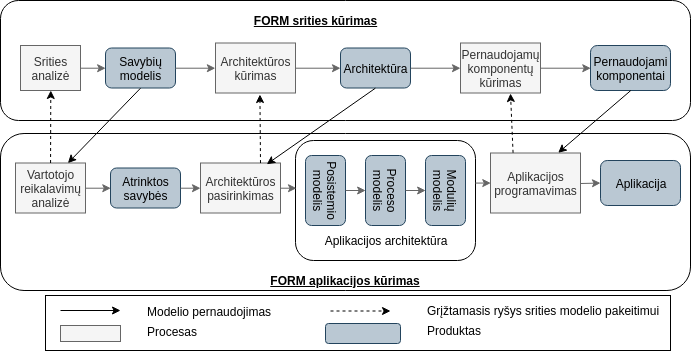
\includegraphics[scale=0.6]{img/form}
    \captionof{figure}{FORM kūrimo procesai \cite{Kang}}
    \label{img:form}
\end{center}


\subsection{Srities architektūros ir komponentų kūrimas}

FORM metodas suteikia sluoksninį architektūros karkasą. Remiantis savybių modeliu, hierarchija turi atskirti paslaugas (angl. service), operacijas, srities technologiją ir įgyvendinamus modulius. Pernaudojami artefaktai yra apibūdinami keturiais lygiais: 1) posistemio (angl. subsystem), 2) proceso, 3) modulių, 4) modulių specifikacijos ir įgyvendinimo \cite{Kang1999}. Architektūra yra kuriama atsižvelgiant į tai, ar savybė yra funkcinė ir savybių suskirstymą į keturis lygius pagal jų tipus. Funkcinės savybės yra naudojamos nustatyti reikalingus komponentus, nefunkcinės suskirsto komponentus bei nustato sąryšius tarp jų. Loginės ribos sukurtos savybių modelio turi atitikti fizines ribas architektūroje \cite{Kang}.


\subsubsection{Srities analizė ir  savybių modeliavimas}

Srities analizė susideda iš: planavimo, savybių analizės ir validavimo. Analizės tikslas yra identifikuoti sistemos bendrumus ir skirtumus srityje. Tai padeda identifikuoti savybes, jas klasifikuoti, organizuoti į modelius (plačiau \ref{modeliavimas} skyriuje) \cite{Kang}.


\subsubsection{Posistemio modelis}

Posistemio modelis parodo pagrindines funkcionalumo grupes programų sistemoje, kiekviena jų gali būti išdėstoma skirtingose mašinose.  Savybių pasiskirstymas skirtingose posistemiuose yra aukšto lygio (angl. high-level) veikimo bei operacinėse aplinkose \cite{Lee2000}. Duomenų perdavimas tarp posistemių yra modeliuojamas neužsiblokuojančiais komunikacijos kanalais, laisvai sujungtais pranešimų eile, arba per blokuojamą pranešimų/atsakymų mechanizmą \cite{Kang}.

\subsubsection{Proceso modelis}

Kiekvienas posistemis yra dalinamas į procesus, kuriuose nusakomas procesų veikimas ir sąveika tarp jų \cite{Lee2000}. Posistemis yra išskirstomas į procesus, perskirstančius operacines savybes į paslaugų savybes. Kiekvienas procesas gali būti skirstomas į ilgalaikį arba trumpalaikį bei į daugkartinį arba ne \cite{Kang}. Posistemio ir proceso modeliai paslaugų savybes paskirsto į lengvai suskirstomus komponentus. Šios paslaugų savybės turi būti įgyvendintos kaip modulių rinkinys \cite{Kang1999}.

\subsubsection{Modulių modelis}

Kiekvienas procesas proceso modelyje yra toliau tobulinamas taip, kad būtų galima sukurti daugkartinio pernaudojimo komponentus - modulius. Modulių hierarchija atitinka savybių hierarchiją savybių modelyje \cite{Lee2000}. Svarbu paminėti, kad hierarchija atskiria modulius, kurie įgyvendina savybes, kurios dažnai keičiasi, nuo žemesnio lygio operacijų ir įgyvendinimo metodų \cite{Kang1999}. Pasirenkamos savybės turi būti įgyvendintos kaip šablono (angl. template) modulis ar aukštesnio lygio modulis su sąsaja, kuri padengtų visus galimus pasirinkimus \cite{Kang}.

\subsection{Aplikacijos kūrimas}

FORM aplikacijos kūrimas yra procesas, kurio metu naudojantis žiniomis apie sritį bei srities architektūrą, sukuriama aplikacija. Aplikacijos kūrimas prasideda nuo vartotojo reikalavimo surinkimo, pagal tai pasirenkant savybes iš savybių modelio, nustatant atitinkamus modelius bei kuriama aplikacija pasinaudojus pernaudojamais srities komponentais \cite{Kang}.

\subsubsection{Reikalavimų analizė ir savybių pasirinkimas}


Aplikacijos kūrimas prasideda nuo vartotojo reikalavimų analizavimo bei atitinkamų savybių suradimo modelyje. Savybių modelis ne tik nurodo galimas sistemos charakteristikas, bet ir apibrėžia tarpusavio santykius bei pasirinkimo kriterijus. Efektyvus metodas rasti tinkamoms savybėms yra pirmiausia apsvarstyti veikimui reikalingas savybes, tada operacinę aplinką ir srities technologijas bei jų įgyvendinimo būdus. Kiekvienas lygis suteikia daugiau detalumo, taip atspindi laipsnišką tobulinimą \cite{Kang}.


\subsubsection{Architektūrinio modelio pasirinkimas ir programavimas}

Savybių pasirinkimo etape automatiškai yra gaunamas atitinkamas architektūrinis modelis. Kai architektūra yra žinoma, pernaudojami komponentai yra lengvai randami (galima pasinaudoti prieš tai suprogramuotais komponentais, užpildyti skeletą ar parametrizuoti šablonus) \cite{Kang}. Taip pasinaudojus srities architektūra lengvai gaunama aplikacijos architektūra bei jos kodas.










%%%%%%%%%%%%%%%%%%%%%%%%%%%%%%%%%%%%%%%%%%%%%%%%%%%%%%%%%%%%%%%%%%%%%%%%%%%%%%%%%%%%%%%%%%%%%%%%%%%
%%%%%%%%%%%%%%%%%%%%%%%%%%%%%%%%%%%%%%%%%%%%%%%%%%%%%%%%%%%%%%%%%%%%%%%%%%%%%%%%%%%%%%%%%%%%%%%%%%%
%%%%%%%%%%%%%%%%%%%%%%%%%%%%%%%%%%%%%%%%%%%%%%%%%%%%%%%%%%%%%%%%%%%%%%%%%%%%%%%%%%%%%%%%%%%%%%%%%%%
%%%%%%%%%%%%%%%%%%%%%%%%%%%%%%%%%%%%%%%%%%%%%%%%%%%%%%%%%%%%%%%%%%%%%%%%%%%%%%%%%%%%%%%%%%%%%%%%%%%
%%%%%%%%%%%%%%%%%%%%%%%%%%%%%%%%%%%%%%%%%%%%%%%%%%%%%%%%%%%%%%%%%%%%%%%%%%%%%%%%%%%%%%%%%%%%%%%%%%%
%%%%%%%%%%%%%%%%%%%%%%%%%%%%%%%%%%%%%%%%%%%%%%%%%%%%%%%%%%%%%%%%%%%%%%%%%%%%%%%%%%%%%%%%%%%%%%%%%%%
%%%%%%%%%%%%%%%%%%%%%%%%%%%%%%%%%%%%%%%%%%%%%%%%%%%%%%%%%%%%%%%%%%%%%%%%%%%%%%%%%%%%%%%%%%%%%%%%%%%
%%%%%%%%%%%%%%%%%%%%%%%%%%%%%%%%%%%%%%%%%%%%%%%%%%%%%%%%%%%%%%%%%%%%%%%%%%%%%%%%%%%%%%%%%%%%%%%%%%%
%%%%%%%%%%%%%%%%%%%%%%%%%%%%%%%%%%%%%%%%%%%%%%%%%%%%%%%%%%%%%%%%%%%%%%%%%%%%%%%%%%%%%%%%%%%%%%%%%%%
%%%%%%%%%%%%%%%%%%%%%%%%%%%%%%%%%%%%%%%%%%%%%%%%%%%%%%%%%%%%%%%%%%%%%%%%%%%%%%%%%%%%%%%%%%%%%%%%%%%
%%%%%%%%%%%%%%%%%%%%%%%%%%%%%%%%%%%%%%%%%%%%%%%%%%%%%%%%%%%%%%%%%%%%%%%%%%%%%%%%%%%%%%%%%%%%%%%%%%%
%%%%%%%%%%%%%%%%%%%%%%%%%%%%%%%%%%%%%%%%%%%%%%%%%%%%%%%%%%%%%%%%%%%%%%%%%%%%%%%%%%%%%%%%%%%%%%%%%%%
%%%%%%%%%%%%%%%%%%%%%%%%%%%%%%%%%%%%%%%%%%%%%%%%%%%%%%%%%%%%%%%%%%%%%%%%%%%%%%%%%%%%%%%%%%%%%%%%%%%



\section{Savybių modeliavimas ICO išmaniesiems kontraktams}

Buvo pasirinkta atlikti savybių modeliavimą remiantis procesu aprašytu \ref{procesas}. skyriuje. Savybių modeliavimas pradėtas nuo srities nusistatymo (plačiau \ref{sritis}. Srities identifikavimas). Toliau, buvo sudaryti trys savybių modeliai: 1) ICO išmaniesiems kontraktams, patalpintiems Ethereum blockchain, 2) OpenZeppelin bibliotekai, 3) TokenMarket bibliotekai. OpenZeppelin ir TokenMarket - atviro kodo Ethereum išmaniųjų kontraktų bibliotekos, populiariausios GitHub\footnote{\url{https://github.com/}} versijų valdymui skirtame tinklapyje. Kiekvieno savybių modelio sudarymas susideda iš: savybių identifikavimo, jų abstrakcijos, klasifikacijos ir modeliavimo bei savybių modelio validacijos.

\subsection{Srities identifikavimas} \label{sritis}

Šio savybių modeliavimo sritis - išmanieji kontraktai pirminiam kriptovaliutų platinimui. Kaip jau buvo minėta įvade: „Per trumpą laiką buvo sukurta daug panašių išmaniųjų kontraktų, kurie dažnai kuriami kopijuojant jau esamus ICO išmaniuosius kontraktus bei pridedant reikiamus pakeitimus. Taip sukurta didelė aibė ICO išmaniųjų kontraktų, kurių kodas yra labai panašus arba kartojasi. Pernaudojamumo problemą išspręsti bandoma Ethereum išmaniųjų kontraktų bibliotekomis, tačiau jos ne visada padengia visą ICO išmaniųjų kontraktų savybių aibę." Todėl norint apžvelgti, kurias ICO išmaniųjų kontraktų savybes bibliotekos padengia, tiriami ICO išmanieji kontraktai, patalpinti Ethereum blockchain bei OpenZeppelin ir TokenMartket bibliotekose.

\subsection{Savybių modeliavimas ICO išmaniesiems kontraktams, patalpintiems Ethereum blockchain}

Pirmiausia tirtos savybės, kurias turi ICO išmanieji kontraktai, patalpinti Ethereum blockchain. Išmaniųjų kontraktų savybės tirtos surinkus aibę ICO išmaniųjų kontraktų. Išanalizavus jų savybes sudarytas savybių modelis bei patikrintas jo validumas.


\subsubsection{Savybių identifikavimas} \label{identifikavimas_eth}

%%%%%NEW%%%%

Savybių modelio sukūrimui yra būtinas savybių identifikavimas. Remiantis \ref{identifikavimas} skyriuje aprašytais savybių identifikavimo būdais buvo pasirinktas jau parašytų programų (šiuo atveju išmaniųjų kontraktų) surinkimas, analizavimas ir savybių juose identifikavimas. Išmaniųjų kontraktų surinkimo procesas:
\begin{enumerate}[topsep=0pt,itemsep=-1ex,partopsep=1ex,parsep=1ex]
\item Sukurtas interneto skaitytuvas\footnote{Interneto skaitytuvas patalpintas: \url{https://github.com/maciukaite/bakalauro-darbas/tree/master/crawler}} (angl. web crawler) naudojantis Node.js karkasu. Jis nuskaito visus išmaniuosius kontraktus, patalpintus ethrescan.io su žyma Token Sale\footnote{\url{https://etherscan.io/accounts/label/token-sale}}(liet. žetonų pardavimas) bei turinčius daugiau nei 700 transakcijų;
\item Visi surinktų išmaniųjų kontraktų Solidity kodai buvo surašyti į failus. Failo pavadinimo struktūra: contract + identifikacijos numeris + .sol plėtinys;
%\item Sukurtas meta duomenų failas, kuriame patalpinta: kiekvieno išmanaus kontrakto adresas, tranzakcijų kiekis bei identifikacinis numeris.
\end{enumerate}

Tokiu būdu buvo surinkta 161 pirminio kriptovaliutų platinimo išmaniųjų kontraktų. Iš jų atrinkta 40 ICO išmaniųjų kontraktų, kurie realizuoja tik ICO funkcionalumą (nerealizuoja žetono funkcionalumo). Išanalizavus atrinktus išmaniuosius kontraktus buvo išskirtos savybės ir apibūdintos dalinai naudojantis forma pateikta FODA \cite{Kang1990}. Visos savybės pateiktos \ref{table:features}-oje lentelėje, pilna lentelės versija pateikta priede \ref{appendix:features}. \ref{table:features}-oje lentelėje nurodytas tik skaičius ICO išmaniųjų kontraktų, patalpintų Ethereum, įgyvendinusių savybę. Prieduose numeriai atitinka surinktų ICO išmaniųjų kontraktų numerius.




\subsubsection{Savybių abstrakcija, klasifikacija, modeliavimas} \label{modelis}

Savybių modelis ICO išmaniesiems kontraktams, patalpintiems Ethereum blockchain (\ref{img:fm_eth} pav.), buvo sukurtas naudojantis savybėmis, kurias turi šie kontraktai. Visos savybės yra pateiktos \ref{table:features}-ioje lentelėje. Savybių pavadinimai modelyje gali nesutapti su pavadinimais lentelėje, tačiau numeracija sutampa. Jei savybė lentelėje neturėjo sau priešingos, tai modelyje priešinga savybė jau yra įvardinama ir tai priimtina kaip savaime suprantamas reiškinys. Tokioms savybėms taip pat suteikta numeracija. Savybės, kurios yra tarp 90\% ir daugiau išmaniųjų kontraktų, yra laikomas privalomomis. Modelyje nėra savybių, kurias turi tik 5\% ir mažiau išmaniųjų kontraktų, tokios savybės laikomos pavienėmis ir dėl tos priežasties nėra įtrauktos į bendrą modelį. Visos savybės modelyje buvo klasifikuotos ir struktūrizuotos naudojant „susideda iš" santykį. Savybės modelyje identifikuotos naudojantis santykių kategorijomis tarp savybių (\ref{img:fm_rules} pav.).

Modelio kompozicijos taisyklės:
\begin{enumerate}[topsep=0pt,itemsep=-1ex,partopsep=1ex,parsep=1ex]
\item Žetonų susigrąžinimui (S2) reikalingas savininkas (S1);
\item Platinimo periodo keitimui bei pradėjimui (S7, S9, S8) reikalingas savininkas (S1);
\item Platinimo periodo laikinam sustabdymui (S3) reikalingas savininkas (S1);
\item Kainos pakeitimui, iškvietus funkciją, (S20) reikalingas savininkas (S1);
\item Žetonus atsiimti po ICO (S29) gali tik investuotojas (S13);
\item ETH susigrąžinti nepasiekus tikslo (S33) gali tik investuotojas (S13);
\item Investuotojų sąrašas egzistuoja tik tada (S38, S14), kai yra identifikuoti investuotojai (S12).
\end{enumerate}
\subsubsection{Savybių modelio validacija} \label{validacija}

Remiantis \ref{validacija_teor}. skyriuje aprašytu procesu validuoti modelį turėtų srities ekspertai ar naujas dokumentų rinkinys. Kadangi šiame darbe negalima pasinaudoti srities ekspertais, tai validacijai naudojami dokumentai - išmanieji kontraktai, kurie buvo surinkti anksčiau (plačiau \ref{identifikavimas_eth}. skyriuje). Iš dar nenaudotų dokumentų buvo atsitiktinai atrinkta 10 išmaniųjų kontraktų ir patikrinta ar savybių modelis (\ref{img:fm_eth} pav.) yra validus. Validacijos rezultatas pateiktas lentelėje:
\begin{center}
    \captionof{table}{ICO savybių modelio validacija}
    \begin{longtable}[H]{| p {3cm} | p{8cm} | p{2.5cm} |}
    \hline
    \textbf{ICO išmanaus kontrakto numeris}  & \textbf{Savybės} & \textbf{Validumas} \endhead \hline

	1 & S10, S1, S25, S18, S7, S3, S9, S2, S39, S28, S37
& validus
 \\
	\hline
	20 & S10, S1, S3, S6, S12, S18, S2, S27, S14, S28, S25, S8 & validus
	\\
		\hline
	33 & S1, S25, S6, S8, S21, S22, S28, S27,S37, S19 & validus
	\\
		\hline
	67 & S1, S25, S21, S18, S20, S3, S27, S6, S36, S37, S28 & validus
	\\
		\hline
	87 &  S1, S25, S6, S36, S18, S21, S3, S27, S37, S28 & validus
	\\
		\hline
	99 &  S1, S25, S21, S18, 36, S6, S3, S27, S28, S9 & validus
	\\
		\hline
	126 &  S1, S25, S27, S36, S6, S37, S28, S19 & validus
	\\
		\hline
	130 &  S1, S25, S27, S36, S6, S37, S28, S19 & validus
	\\
		\hline
	145 & S1, S25, S27, S36, S6, S37, S28, S19 & validus
	\\
		\hline
	160 &  S1, S25, S39, S36, S6, S3, S12, S14, S29, S18, S22, S21 & validus
	\\
		\hline


\end{longtable}
    \label{table:validacija}

\end{center}
\pagebreak

\begin{landscape}

\begin{center}
    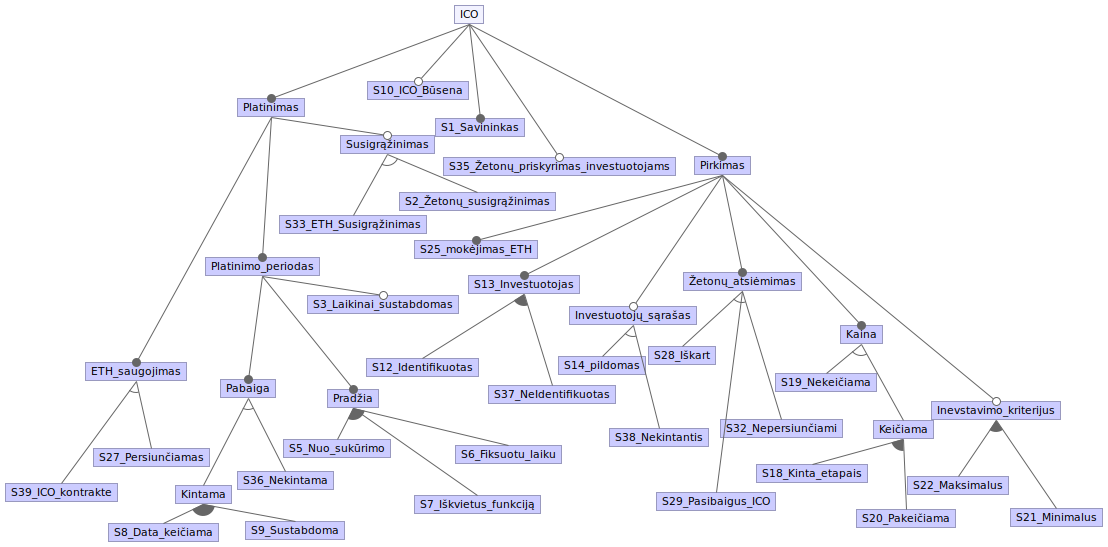
\includegraphics[scale=0.7]{img/eth_feature_model}
    \captionof{figure}{Savybių modelis ICO išmaniesiems kontraktams, patalpintiems Ethereum blockchain}
    \label{img:fm_eth}
\end{center}

\end{landscape}
%\pagebreak




\subsection{Savybių modeliavimas OpenZeppelin ICO išmaniesiems kontraktams}

OpenZeppelin - atviro kodo Ethereum išmaniųjų kontraktų biblioteka, populiariausia GitHub tinklapyje. OpenZeppelin biblioteka suteikia daug įvairių Ethereum išmaniųjų kontraktų. Šiam darbui pasirinkti tik tie išmanieji kontraktai, kurie realizuoja ICO arba yra tiesiogiai susiję su ICO išmaniaisiais kontraktais. Išanalizuotos tų kontraktų savybės bei sudarytas savybių modelis. Kadangi analizuojamos bibliotekos savybės, tai savybių modelio validacija nėra atliekama.

\subsubsection{Savybių identifikavimas}

Savybių identifikavimas OpenZeppelin bibliotekai buvo atliktas pasirinkus išmaniuosius kontraktus, kurie įgyvendina ICO funkcionalumą arba yra tiesiogiai su juo susiję. OpenZeppelin biblioteka yra patalpinta versijavimo sistemoje, pasirinkta specifinė kontraktų versija - darbo rašymo metu naujausia versija. Pasirinkta versija - 81e36d2e74ee8218339028bdf97a4e9116a5da6a\footnote{Nuoroda į pasirinktą OpenZeppelin bibliotekos versiją: \url{https://github.com/OpenZeppelin/openzeppelin-solidity/tree/81e36d2e74ee8218339028bdf97a4e9116a5da6a}}. Šios savybės taip pat pateiktos \ref{table:features}-oje lentelėje, pilna lentelės versija pateikta priede \ref{appendix:features}. \ref{table:features}-oje lentelėje OpenZeppelin stulpelyje pateiktas faktas, ar biblioteka savybę įgyvendina. Prieduose pateikti išmanieji kontraktai turintys atitinkamas savybes. Pilna nuoroda iki išmanaus kontrakto: nuoroda į bibliotekos versiją + /contracts/crowdsale + /OpenZeppelin išmanusis kontraktas + .sol\footnote{Pavyzdžiui, \url{https://github.com/OpenZeppelin/openzeppelin-solidity/blob/81e36d2e74ee8218339028bdf97a4e9116a5da6a/contracts/crowdsale/Crowdsale.sol}}.

\subsubsection{Savybių abstrakcija, klasifikacija, modeliavimas}

Savybių modelis OpenZeppelin ICO išmaniesiems kontraktams (\ref{img:fm_oz} pav.) buvo sukurtas naudojantis savybėmis, kurias turi šie kontraktai. Visos savybės yra pateiktos \ref{table:features}-je lentelėje. Savybių abstrakcijos, klasifikacijos ir modeliavimo procesas nesiskyrė nuo proceso pateikto \ref{modelis} skyriuje. Modelio kompozicijos taisyklės:
\begin{enumerate}[topsep=0pt,itemsep=-1ex,partopsep=1ex,parsep=1ex]
\item Platinimo periodo pabaigos datos keitimui (S8) reikalingas savininkas (S1);
\item Platinimo periodo laikinam sustabdymui (S3) reikalingas savininkas (S1);
\item Žetonus atsiimti po ICO (S29) gali tik investuotojas (S12, S37);
\item ETH susigrąžinti nepasiekus tikslo (S33) gali tik investuotojas (S12, S37);
\item Investuotojų sąrašas egzistuoja tik tada (S38, S14, S15), kai yra identifikuoti investuotojai (S12).
\end{enumerate}
\pagebreak

\begin{landscape}

\begin{center}
    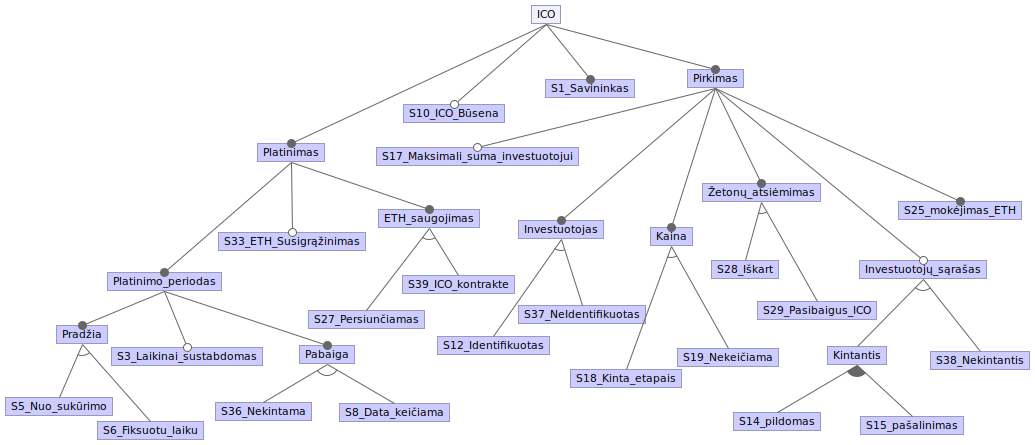
\includegraphics[scale=0.7]{img/oz_feature_model}
    \captionof{figure}{Savybių modelis OpenZeppelin ICO išmaniesiems kontraktams}
    \label{img:fm_oz}
\end{center}

\end{landscape}


\subsection{Savybių modeliavimas TokenMarket ICO išmaniesiems kontraktams}

TokenMarket - antra pagal populiarumą Ethereum išmaniųjų kontraktų biblioteka GitHub. Savybių modeliavimui pasirinkti tik tie išmanieji kontraktai, kurie įgyvendina ICO funkcionalumą arba yra tiesiogiai susiję su ICO išmaniaisiais kontraktais. Išanalizavus savybes, sudarytas bibliotekos savybių modelis. Kadangi analizuojamos bibliotekos savybės, tai savybių modelio validacija nėra atliekama. Nėra būdo atlikti validaciją bibliotekoms, nes nebuvo galimybės pasitelkti srities ekspertais, kurie nedalyvavo modeliavime, taip pat nėra naujo aplikacijų rinkinio, kuris galėtų būti naudojamas validacijai.

\subsubsection{Savybių identifikavimas}

Pasirinkti visi TokenMarket patalpinti išmanieji kontraktai, kurie įgyvendina ICO funkcionalumą arba yra tiesiogiai su juo susiję. TokenMarket bibliotekos analizavimui pasirinkta 067e241dffb7c7865b0f7628a875d285c7cd894c \footnote{Nuoroda į pasirinktą TokenMarket bibliotekos versiją: \url{https://github.com/TokenMarketNet/smart-contracts/tree/067e241dffb7c7865b0f7628a875d285c7cd894c}} versija. Visos savybės pateiktos \ref{table:features}-oje lentelėje (pilna lentelės versija pateikta priede \ref{appendix:features}). \ref{table:features}-oje lentelėje pateiktas faktas apie  savybės įgyvendinimą bibliotekoje. Prieduose TokenMarket stulpelyje pateikti išmanieji kontraktai turintys atitinkamas savybes. Pilna nuoroda iki išmanaus kontrakto: nuoroda į bibliotekos versiją + /contracts + /TokenMarket išmanusis kontraktas + .sol\footnote{Pavyzdžiui, \url{https://github.com/TokenMarketNet/smart-contracts/blob/067e241dffb7c7865b0f7628a875d285c7cd894c/contracts/CrowdsaleBase.sol}}.

\subsubsection{Savybių abstrakcija, klasifikacija, modeliavimas}

Savybių modelis TokenMarket ICO išmaniesiems kontraktams (\ref{img:fm_tm} pav.) buvo sukurtas naudojantis savybėmis, kurias turi šie kontraktai. Visos savybės yra pateiktos \ref{table:features}-ioje lentelėje. Savybių abstrakcijos, klasifikacijos ir modeliavimo procesas nesiskyrė nuo proceso pateikto \ref{modelis} skyriuje. Modelio kompozicijos taisyklės:
\begin{enumerate}[topsep=0pt,itemsep=-1ex,partopsep=1ex,parsep=1ex]
\item Platinimo periodo keitimui (S9, S8) reikalingas savininkas (S1);
\item Platinimo periodo laikinam sustabdymui (S3) reikalingas savininkas (S1);
\item Žetonus atsiimti po ICO (S29) gali tik investuotojas (S13);
\item ETH susigrąžinti nepasiekus tikslo (S33) gali tik investuotojas (S13);
\item Investuotojų sąrašas egzistuoja tik tada (S38, S14), kai yra identifikuoti investuotojai (S12).
\end{enumerate}

\pagebreak

\begin{landscape}

\begin{center}
    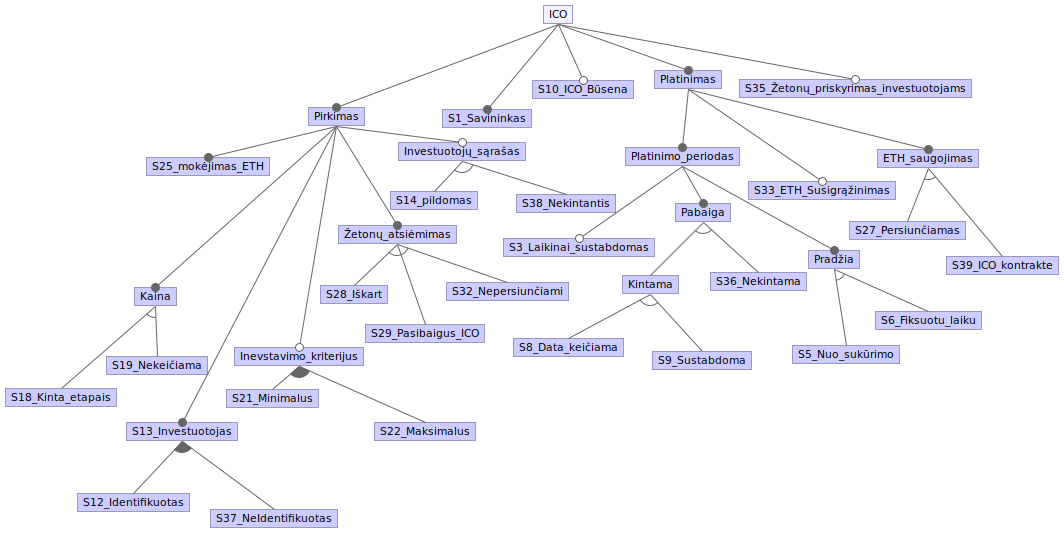
\includegraphics[scale=0.7]{img/tm_feature_model}
    \captionof{figure}{Savybių modelis TokenMarket ICO išmaniesiems kontraktams}
    \label{img:fm_tm}
\end{center}

\end{landscape}

\pagebreak
	\begin{center}
    \captionof{table}{ICO išmaniųjų kontraktų savybių įgyvendinimas}
    \begin{longtable}[H]{| p {6.1cm} | p{2.6cm} | p{2.6cm} | p{2.6cm} |}
    \hline
    \textbf{Savybės pavadinimas }  & \textbf{Ethereum ICO išmaniųjų kontraktų skaičius} & \textbf{Įgyvendinta OpenZeppelin bibliotekoje} & \textbf{Įgyvendinta TokenMarket bibliotekoje} \endhead \hline

    S1. Savininkas  & 36 & + &  + \\ \hline

S2. Žetonų susigrąžinimas & 8 & - &  - \\ \hline

%pradžia/pabaiga

S3. Laikinas sustabdymas  & 17 & + & + \\ \hline

S4. Pradžios ir pabaigos datos nustatymas tik sukūrus išmanųjį kontraktą \footnote{Ši savybė laikoma paviene ir nėra įtraukta į modelį, nes jos neįgyvendina daugiau nei 5\% išmaniųjų kontraktų\label{neitraukta}}  &  2 & -  & - \\ \hline

S5. ICO pradžia nuo sukūrimo & 5 & + &  + \\ \hline

S6.ICO pradžia fiksuotu laiku & 25 & + & + \\ \hline

S7. ICO prasideda iškvietus funkciją & 6 & - & - \\ \hline

S8. Kintama ICO pabaiga & 10  & + & + \\ \hline

S9. Rankinis ICO sustabdymas & 4 & - & + \\ \hline

%būsena

S10. ICO būsena  & 12 & + & + \\ \hline

S11. Rankinis ICO būsenos pakeitimas\textsuperscript{\ref{neitraukta}}
  & 2 & - & - \\ \hline


%identifikavimas

S12. Identifikuotas investavimas & 3 & + & +\\ \hline

S13. Neidentifikuotas ir identifikuotas investavimas & 10 & - & + \\ \hline

S14. Pildomas identifikuotų investuotojų sąrašas & 7 & + & + \\ \hline

S15. Galimybė pašalinti investuotoją\textsuperscript{\ref{neitraukta}}
 & 1 & + & -\\ \hline


S16. Galimybė investuoti kitu adresu\textsuperscript{\ref{neitraukta}}
  & 1 & - & - \\ \hline

S17. Maksimali investavimo suma investuotojui & 0 & + & -\\ \hline

%Kaina

S18. Kintanti kaina &  19 & + & + \\ \hline

S19. Nekintanti kaina & 12 & + & + \\ \hline

S20. Pakeičiama kaina  & 8 & - & - \\ \hline

%pirkimo sąlygos

S21. Minimalus investavimas & 13 & - & +\\ \hline

S22. Maksimalus investavimas & 8 & - & + \\ \hline

S23. Kintanti bendra investavimo suma\textsuperscript{\ref{neitraukta}}
 &  1 & - & - \\ \hline
%Ether

S24. Žetonų pirkimas netiesiogiai\textsuperscript{\ref{neitraukta}}
 & 2 & - & - \\ \hline

S25. Žetonų pirkimas tiesiogai & 37 & + & +\\ \hline

S26. Žetonų pirkimas investavus BTC ar ETH\textsuperscript{\ref{neitraukta}}
 & 1 & - & - \\ \hline


S27. Visi ETH yra iš karto persiunčiami &  13 & + & +\\ \hline

%žetonų atsiėmimas

S28. Žetonų persiuntimas iš karto & 24 & + & + \\ \hline


S29. Žetonų atsiėmimas pasibaigus ICO & 9 & + & + \\ \hline

S30. Žetonų atsiėmimas pasibaigus ICO, su savininko atrakinimu\textsuperscript{\ref{neitraukta}}
 & 1 & - & - \\ \hline

S31. Žetonai persiunčiami savininko\textsuperscript{\ref{neitraukta}}
 & 1 & - & -\\ \hline

S32. Žetonai nepersiunčiami &  8 & - & + \\ \hline

%pabaigos sąlygos


S33. ETH susigrąžinimo galimybė  & 14  & +  & + \\	\hline


%partneriai

S34. Žetonų padalijimas partneriams\textsuperscript{\ref{neitraukta}}
& 1 & - & - \\ \hline

S35. Žetonų priskyrimas investuotojams & 4 & - & + \\ \hline


    \end{longtable}
        \label{table:features}
    	\addtocounter{table}{-1}

\end{center}

\section{ICO savybių modelių palyginimas} \label{palyginimas}

Savybių modeliai palyginti remiantis sukurtais modeliais (modeliai pavaizduoti \ref{img:fm_eth}, \ref{img:fm_oz}, \ref{img:fm_tm} paveikslėliuose). OpenZeppelin ir TokenMarket modeliai lyginti su ICO išmaniųjų kontraktų, patalpintų Ethereum blockchain, modeliu. Palyginti savybių skirtumai tarp šių modelių, išskirtos savybės, kurios modeliuose nesutampa.


\subsection{Palyginimas su OpenZeppelin}

Savybės, kurias turi ICO išmanieji kontraktai, patalpinti Ethereum blockchain, bet neturi OpenZeppelin ICO išmanieji kontraktai:
\begin{enumerate}[topsep=0pt,itemsep=-1ex,partopsep=1ex,parsep=1ex]
\item S2. Žetonų susigrąžinimas;
\item S7. ICO prasideda iškvietus funkciją;
\item S9. Rankinis ICO sustabdymas;
\item S13. Neidentifikuotas ir identifikuotas investavimas;
\item S20. Pakeičiama kaina;
\item S21. Minimalus investavimas;
\item S22. Maksimalus investavimas;
\item S32. Žetonai nepersiunčiami;
\item S35. Žetonų priskyrimas investuotojams.
\end{enumerate}


Savybės, kurias turi OpenZeppelin ICO išmanieji kontraktai, bet neturi ICO išmanieji kontraktai, patalpinti Ethereum blockchain:
\begin{enumerate}[topsep=0pt,itemsep=-1ex,partopsep=1ex,parsep=1ex]
\item S17. Maksimali investavimo suma investuotojui.
\end{enumerate}


\subsection{Palyginimas su TokenMarket} \label{tm:palyginimas}

Savybės, kurias turi ICO išmanieji kontraktai, patalpinti Ethereum blockchain, bet neturi TokenMarket ICO išmanieji kontraktai:
\begin{enumerate}[topsep=0pt,itemsep=-1ex,partopsep=1ex,parsep=1ex]
\item S2. Žetonų susigrąžinimas;
\item S7. ICO prasideda iškvietus funkciją;
\item S20. Pakeičiama kaina.
\end{enumerate}

                                                                                                                                                                                                                                Nėra savybių, kurias turi TokenMarket ICO išmanieji kontraktai, bet neturi ICO išmanieji kontraktai, patalpinti Ethereum blockchain.

\section{Pasiūlymai TokenMarket bibliotekai}


Atsižvelgus į \ref{palyginimas} skyrių buvo nuspręsta daryti palyginimus TokenMarket bibliotekai. Ši biblioteka pasirinkta, nes ji turi mažiau savybių nesutampančių su ICO išmaniaisiais kontraktais, patalpintais Ethereum blockchain - biblioteka labiau padengianti realų savybių poreikį.

Pasiūlymų teikimo procesas susideda iš: savybių surikiavimo pagal svarbumą, patikrinimo, ar savybės nebuvo įgyvendintos nuo to laiko, kai savybių modeliavimas buvo atliktas arba ar nėra pateikti pasiūlymai šių savybių įgyvendinimui, pasiūlymų įgyvendinti reikiamas savybes.


\subsection{Savybių svarbumas}

Visos trūkstamos savybės (jos yra pateiktos \ref{tm:palyginimas} skyriuje) pirmiausiai surikiuotos pagal svarbumą (svarbumas skirstomas pagal išmaniuosius kontraktus, kurie yra įgyvendinę šias savybes (informacija apie savybių įgyvendinimą išmaniuose kontraktuose pateikta \ref{table:features} lentelėje)), svarbiausia savybė - įgyvendinta daugiausiai išmaniųjų kontraktų). Savybės pagal svarbumą:
\begin{enumerate}[topsep=0pt,itemsep=-1ex,partopsep=1ex,parsep=1ex]
\item S2. Žetonų susigrąžinimas (įgyvendinta 8-iuose išmaniuosiuose kontraktuose);
\item S20. Pakeičiama kaina (įgyvendinta 8-iuose išmaniuosiuose kontraktuose);
\item S7. ICO prasideda iškvietus funkciją (įgyvendinta 6-iuose išmaniuosiuose kontraktuose).
\end{enumerate}



\subsection{Savybių statuso patikrinimas naujausioje bibliotekos versijoje}

Savybių modeliavimui buvo pasirinkta specifinė šios bibliotekos versija. Nuo to laiko, kai savybių modeliavimas buvo atliktas, atsirado ne viena nauja bibliotekos versija. Tam, kad būtų užtikrintas savybių ir kodo nesikartojimas, pirmiausia patikrinta naujausia bibliotekos versija  darbo rašymo metu - 2c5b78d8e4f5d272f0eacba487f00408a36dfb95\footnote{Nuoroda į pasirinktą TokenMarket bibliotekos versiją: \url{https://github.com/TokenMarketNet/smart-contracts/tree/2c5b78d8e4f5d272f0eacba487f00408a36dfb95}}. Taip pat patikrinti atviri prašymai pakeitimams (angl. pull request) ir iškeltos problemos (angl. issue) pateikti iki 2019-05-08 dienos.

Pirmiausia tikrinti pasikeitimai pagrindinėje (angl. master) bibliotekos šakoje (angl. branch). Patikrinti pasikeitimai pagrindinėje šakoje nuo tos versijos, kuri naudota savybių modeliavimui. Nustatyta, kad pasikeitimų, kurie galėtų įgyvendinti trūkstamas savybes, neįvyko.

2019-05-08 buvo 8 prašymai pakeitimams ir 20 problemų. Peržiūrėjus visus prašymus pakeitimams ir problemas, nustatyta, kad jie neįgyvendina trūkstamų savybių.


\subsection{Siūlomi pakeitimai TokenMarket bibliotekai}

Siūlomi pakeitimai įgyvendinti dalinai naudojantis FORM (plačiau \ref{form} skyriuje).  Posistemio ir proceso modeliai šiuo atveju yra neaktualūs, nes nebuvo tirta aplinka, su kuria išmanieji kontraktai sąveikauja, tirtas tik jų veikimas Ethereum blockhain. Nubraižytas TokenMarket ICO išmaniųjų kontraktų modulių modelis, jis papildytas naujai pridėtais išmaniaisiais kontraktais po pasiūlymų pateikimo (\ref{img:tm_module} paveikslėlis). Taip pat papildomai nubraižytas savybių pasiskirstymas TokenMarket ICO išmaniuosiuose kontraktuose po pasiūlymų (\ref{img:tm_features} paveikslėlis).

%Visiems pasiūlymams sukurtos problemos bibliotekos saugykloje (angl. repository) GitHub. Taip sukurti prašymai pakeitimams.

% Modulių modelis aktualus, tačiau ne visai bibliotekos architektūrai, bet atskiroms savybėms, kurias ruošiamasi įgyvendinti. Modulių modelio bibliotekai nuspręsta nebraižyti, nes tai turi būti atliekama pačių bibliotekos kūrėjų ir darbo apimtis neapima visos bibliotekos analizavimo iš architektūros pusės. Kiekvienai siūlomai įgyvendinti savybei nubraižytas modulių modelis, kuriame atvaizduotos alternatyvios savybės bei galimi pasirinkimai tarp savybių. Nubraižius modulių modelį iškelta problema bibliotekoje bei pasiūlomas pakeitimas bibliotekai bibliotekos saugykloje (angl. repository) GitHub.


\subsubsection{S2. Žetonų susigrąžinimas} \label{suggestions:s2}

Žetonų susigrąžinimo savybę nuspręsta įgyvendinti CrowdsaleBase išmaniajame kontrakte. Remiantis savybių modeliu ši savybė neprieštaraus jau esančiomis savybėmis, o tik praplės CrowdsaleBase funkcionalumą. Taip pat didelė dalis išmaniųjų kontraktų, kurie įgyvendino savybes esančias CrowdsaleBase, turėjo žetonų susigrąžinimo funkcionalumą.

TokenMarket GitHub saugykloje sukurta problema numeris 159\footnote{Nuoroda į problemą 159 TokenMarket bibliotekoje: \url{https://github.com/TokenMarketNet/smart-contracts/issues/159}}. Problema apibūdina atliktą tyrimą ir tai, kad jo metu nustatyta - žetonų susigrąžinimo savybė nėra įgyvendinta bibliotekoje. Taip pat pasiūlytas galimas kodas žetonų susigrąžinimo savybei. Kodas realizuotas bibliotekoje ir pasiūlytas pakeitimas bibliotekai\footnote{Nuoroda į pasiūlymą TokenMarket bibliotekoje: \url{https://github.com/TokenMarketNet/smart-contracts/pull/1629}} kartu su kitomis trūkstamomis savybėmis.

Žetonų susigrąžinimo savybės įgyvendinimui buvo sukurta viena funkcija (ji pateikta \ref{code:s2} paveikslėlyje). Ji sukurta naudojantis kodu, kuris buvo naudojamas tai pačiai savybei kituose išmaniuosiuose kontraktuose. Ši funkcija pridėta prie CrowdsaleBase išmanaus kontrakto.


\begin{figure}[H]
    \small
	\begin{lstlisting}
  function withdrawTokens ( address _token , address to , uint256 amount )
  public
  onlyOwner
  {
    FractionalERC20 token = FractionalERC20(_token);

    if(!token.transfer(to , amount )) throw ;
  }
\end{lstlisting}
	\caption{Žetonų susigrąžinimo savybės įgyvendinimas CrowdsaleBase išmaniajame kontrakte}
	\label{code:s2}
\end{figure}

\subsubsection{S20. Pakeičiama kaina}

Pakeičiamos kainos savybę nuspręsta pridėti prie MilestonePricing išmaniojo kontrakto. Toks pasirinkimas priimtas, nes šios savybės turi bendrą tėvinį mazgą ir 7/8 išmaniųjų kontraktų, kurie turi šią savybę, taip pat turi ir savybę S18. Kintanti kaina.

Šiai savybei sukurta dar viena problema - 160\footnote{Nuoroda į problemą 160 TokenMarket bibliotekoje: \url{https://github.com/TokenMarketNet/smart-contracts/issues/160}}. Problemas struktūra sutampa su \ref{suggestions:s2} skyriuje apibūdinta problema. Savybės įgyvendinimui buvo sukurta funkcija (ji pateikta \ref{code:s20} paveikslėlyje). Ji sukurta naudojantis kodu, kuris buvo naudojamas tai pačiai savybei kituose išmaniuosiuose kontraktuose bei pritaikyta MilestonePricing. Funkcija pridėta prie MilestonePricing išmanaus kontrakto.

\begin{figure}[H]
    \small
	\begin{lstlisting}
  function setCurrentPrice (uint price) public onlyOwner {
     uint i;

    for(i=0; i<milestones.length; i++) {
      if(now < milestones[i].time) {
        milestones[i-1].price = price;
      }
    }
  }
\end{lstlisting}
	\caption{Pakeičiamos kainos savybės įgyvydendinimas MilestonePricing išmaniajame kontrakte}
	\label{code:s20}
\end{figure}



\subsubsection{S7. ICO prasideda iškvietus funkciją}

ICO prasideda iškvietus funkciją savybei sukurtas naujas išmanusis kontraktas - StartableCrowdsale. Kadangi yra tik vienas kontraktas, kuris turi abi savybes: S7. ICO prasideda iškvietus funkciją ir S6. ICO pradžia fiksuotu laiku. Sudėti šias savybes į vieną išmanųjį kontraktą yra neaktualu, nes dauguma išmaniųjų kontraktų paveldi CrowdsaleBase savybę - S6. ICO pradžia fiksuotu laiku.

Savybei sukurta trečia problema - 161\footnote{Nuoroda į problemą 161 TokenMarket bibliotekoje: \url{https://github.com/TokenMarketNet/smart-contracts/issues/161}}. Problemos struktūra yra tokia pati, kaip kitų dviejų (plačiau \ref{suggestions:s2} skyriuje). Problemai išspręsti sukurtas išmanusis kontraktas  - StartableCrowdsale. Šis išmanusis kontraktas praplečia CrowdsaleBase funkcionalumą bei pridedą funkciją, kuri įgyvendiną ICO prasideda iškvietus funkciją savybę (išmanusis kontraktas pateiktas \ref{code:s7} paveikslėlyje).


\begin{figure}[H]
    \small
	\begin{lstlisting}
import "./CrowdsaleBase.sol";

contract StartableCrowdsale is CrowdsaleBase{

  event StartAtChanged(uint newStartAt);

  constructor  (address _token, PricingStrategy _pricingStrategy,
  address _multisigWallet, uint _start, uint _end, uint _minimumFundingGoal)
    CrowdsaleBase (_token, _pricingStrategy, _multisigWallet,
    _start, _end, _minimumFundingGoal) public{}
    /**
    * @dev Start Crowdsale
    */
    function startCrowdsale () public onlyOwner inState(State.PreFunding){
      startsAt = now;
      StartAtChanged(startsAt);
    }
}

\end{lstlisting}
	\caption{Pakeičiamos kainos savybės įgyvendinimas MilestonePricing išmaniajame kontrakte}
	\label{code:s7}
\end{figure}


\subsection{TokenMarket atsakymas į pasiūlytus pakeitimus}

TokenMarket pateikė atsakymą į prašymą pakeitimui\footnote{Nuoroda į atsakymą: \url{https://github.com/TokenMarketNet/smart-contracts/pull/162#issuecomment-494827821}}. Jie atsakė, kad šiuo metu netęsia ICO išmaniųjų kontraktų kūrimo dėl pasikeitusios rinkos, šiuo metu jie fokusuojasi ties vetybinių popierių žetonų platinimu (angl. security token offering, toliau STO). STO - naujas žetonų platinimo būdas. TokenMarket turi STO kūrimo įrankį\footnote{Nuoroda į TokenMarket STO įrankį: \url{https://github.com/TokenMarketNet/sto}}, kuris leidžia lengvai kurti vertybinių popierių žetonus bei juos platinti keliuose blockchain. Šis įrankis leidžia neturint daug programavimo žinių susikurti žetoną ir jį platinti.



\pagebreak

\begin{landscape}

\begin{center}
    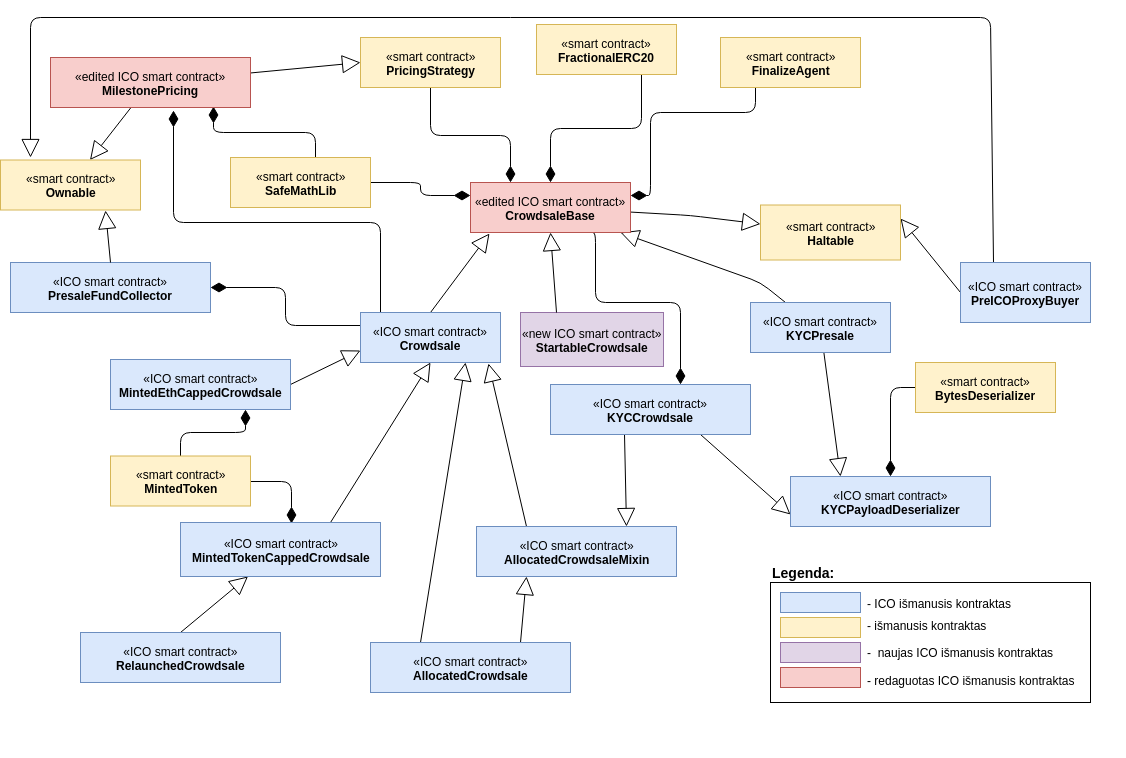
\includegraphics[scale=0.59]{img/tm_moduliai}
    \captionof{figure}{TokenMarket ICO išmaniųjų kontraktų modulių modelis po pasiūlymų pateikimo}
    \label{img:tm_module}
\end{center}

\end{landscape}

\pagebreak

\begin{landscape}

\begin{center}
    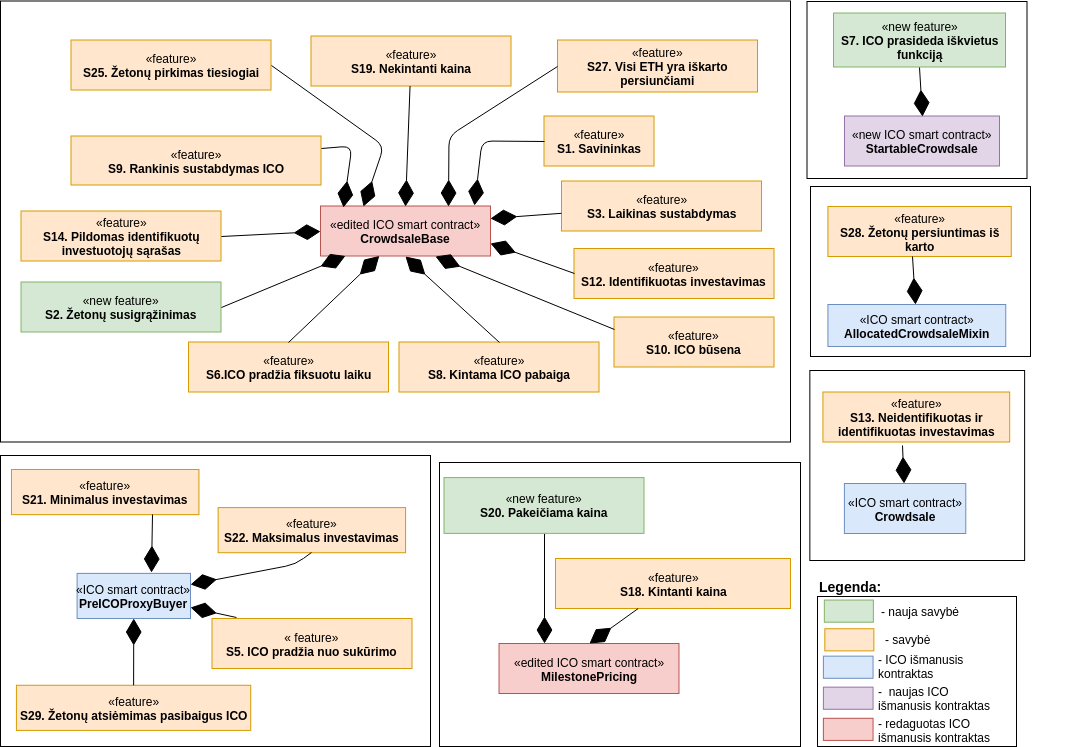
\includegraphics[scale=0.55]{img/tm+savybes}
    \captionof{figure}{Savybių pasiskirstymas TokenMarket ICO išmaniuosiuose kontraktuose po pasiūlymų pateikimo}
    \label{img:tm_features}
\end{center}

\end{landscape}


\sectionnonum{Rezultatai}

Šiame darbe pasiekti rezultatai:
\begin{enumerate}[topsep=0pt,itemsep=-1ex,partopsep=1ex,parsep=1ex]
\item Surinkti 161 ICO išmanieji kontraktai, patalpinti Ethereum blokų grandinėje. Iš jų 40 panaudota išskiriant savybių modelį;
\item Išskirti OpenZeppelin ir TokenMarket ICO išmaniųjų kontraktų savybių modeliai;
\item Palyginti OpenZeppelin ir TokenMarket savybių modeliai su ICO išmaniųjų kontraktų, patalpintų Ethereum blockchain, savybių modeliu;
\item Sukurtos trys problemos TokenMarket bibliotekos GitHub talpykloje. Pasiūlyta, kaip trūkstamas savybes įgyvendinti bibliotekoje.
\end{enumerate}

\bigbreak



Darbo tikslas - patikrinti ar Ethereum bibliotekos padengia visas savybes, kurias turi ICO išmanieji kontraktai patalpinti Ethereum blockchain, bei pasiūlyti būdą ICO išmaniųjų kontraktų kodo pernaudojamumui didinti - pasiektas. Pernaudojamumą bandoma užtikrinti bibliotekomis. Pateikti pasiūlymai TokenMarket bibliotekai leistų padidinti pernaudojamumą ICO išmaniuosiuose kontraktuose.


\sectionnonum{Išvados}

\subsection*{Išvados}

Atlikus darbą daromos išvados:
\begin{enumerate}[topsep=0pt,itemsep=-1ex,partopsep=1ex,parsep=1ex]
\item Savybių modeliavimas yra geras būdas ICO išmaniųjų kontraktų kintamumui ir bendrumui nustatyti. Tačiau savybių pernaudojimo metodas šiai sričiai nevisiškai tinka.  Posistemio ir proceso modeliai neaktualūs ICO išmaniųjų kontraktų sričiai, nors savybių pernaudojamumo metodas nurodo kurti šiuos modelius;
\item Savybių pernaudojimo metodas tyrinėjamas mažai: nedaug susijusių šaltinių, dažniausiai jie seni, dauguma autorių šaltiniuose sutampa;
\item TokenMarket ir OpenZeppelin bibliotekos savybėmis nepilnai padengia savybių, kurias turi ICO išmanieji kontraktai, patalpinti Ethereum blockchain. TokenMarket padengia didesnį savybių kiekį nei OpenZeppelin;
\item ICO evoliucionavo, STO yra naujas žetonų platinimo būdas, kuris galėtų pakeisti ICO. TokenMarket perėjimas prie šio žetonų platinimo būdo, rodo jo potencialą. Toliau plečiant TokenMarket STO įrankį, gali būti, kad ateityje nebereiks turėti daug programavimo žinių sukurti ir platinti žetonus.
\end{enumerate}

\subsection*{Darbo tęsimas}

Darbą toliau galima tęsti šiomis kryptimis:
\begin{enumerate}[topsep=0pt,itemsep=-1ex,partopsep=1ex,parsep=1ex]
\item Būtų galima išplėsti sritį bei tirti ne tik ICO savybes, bet ir žetonų savybes. Taip pat galima tirti sąryšius tarp žetono ir ICO išmaniųjų kontraktų. Taip būtų galima ištirti ir išmaniuosius kontraktus, kurie turi žetono ir ICO funkcionalumą. Kadangi didžioji dauguma išmaniųjų kontraktų šias sritis sujungia kartu (šiame darbe 121 išmanusis kontraktas iš 161 apėmė žetono ir ICO sritis);
\item Būtų galima pasiūlyti naują biblioteką, kuri pilnai remtųsi tik išmaniųjų kontraktų, patalpintų Ethereum blockchain ir savybėmis. Modulių modelis turėtų išplaukti iš savybių modelio, taip būtų galima sukurti biblioteką, kuri būtų visiškai paremta savybių modeliavimu ir savybių pernaudojimo metodu;
\item Būtų galima tęsti darbą STO tema bei palyginti jį su ICO iš savybių modeliavimo pusės. Galima sudaryti STO savybių modelį, palyginti jį su ICO savybių modeliu, nustyti žetonų platinimo būdų skirtumus iš savybių modeliavimo perspektyvos.
\end{enumerate}




%Rezultatų ir išvadų dalyje išdėstomi pagrindiniai darbo rezultatai (kažkas
%išanalizuota, kažkas sukurta, kažkas įdiegta), toliau pateikiamos išvados
%(daromi nagrinėtų problemų sprendimo metodų palyginimai, siūlomos
%rekomendacijos, akcentuojamos naujovės). Rezultatai ir išvados pateikiami
%sunumeruotų (gali būti hierarchiniai) sąrašų pavidalu. Darbo rezultatai turi
%atitikti darbo tikslą.

\printbibliography[heading=bibintoc]  % Šaltinių sąraše nurodoma panaudota
% literatūra, kitokie šaltiniai. Abėcėlės tvarka išdėstomi darbe panaudotų
% (cituotų, perfrazuotų ar bent paminėtų) mokslo leidinių, kitokių publikacijų
% bibliografiniai aprašai. Šaltinių sąrašas spausdinamas iš naujo puslapio.
% Aprašai pateikiami netransliteruoti. Šaltinių sąraše negali būti tokių
% šaltinių, kurie nebuvo paminėti tekste. Šaltinių sąraše rekomenduojame
% necituoti savo kursinio darbo, nes tai nėra oficialus literatūros šaltinis.
% Jei tokių nuorodų reikia, pateikti jas tekste.

%\sectionnonum{Sąvokų apibrėžimai ir santrumpos}

\sectionnonum{Sąvokų apibrėžimai}

Turing pilna (angl. complete) - bet kuri sistema, kuri yra pakankamai universali atpažinti visus galimus algoritmus \cite{Teller1994}.


Interneto skaitytuvas (angl. web crawler) -  programa, kuri nuskaito svetainę ar svetainių rinkinį, analizuoja surinktus puslapius ir praneša apie rezultatus. \cite{Thelwall2001}.


\sectionnonum{Santrumpos}

PLSE - produktų linijos programų inžinerija (angl. product line software engineering).

ICO - pirminis kriptovaliutų platinimas (angl. initial coin offering).

FODA - Feature-Oriented Domain Analysis \cite{Kang1990}.

FORM - savybių pernaudojimo metodas (angl. feature-oriented reuse method).

STO - vertybinių popierių žetonų platinimas (angl. security token offering).


\begin{landscape}

\appendix

\section{ICO išmaniųjų kontraktų savybės} \label{appendix:features}
%% Prieduose gali būti pateikiama pagalbinė, ypač darbo autoriaus savarankiškai
%% parengta, medžiaga. Savarankiški priedai gali būti pateikiami ir
%% kompaktiniame diske. Priedai taip pat numeruojami ir vadinami. Darbo tekstas
%% su priedais susiejamas nuorodomis.
%%\pagebreak
%%\lstinputlisting[language=json]{crawler/res/meta.json}
%

	\begin{center}
    \begin{longtable}[H]{| p {5cm} | p{6.5cm} | p{5.7cm} | p{3.5cm} | p{3.5cm} |}
    \hline
    \textbf{Savybės pavadinimas } &\textbf{Apibūdinimas} & \textbf{Ethereum ICO išmaniųjų kontraktų numeriai} & \textbf{OpenZeppelin išmanieji kontraktai} & \textbf{TokenMarket išmanieji kontraktai} \endhead \hline


%Savininkas
S1. Savininkas & Išmanusis kontraktas turi priviligijuotą adresą - kontrakto savininką, kuris turi daugiau funkcionalumo nei įprastas naudotojas  & 0, 5, 8, 9, 10, 11, 15, 17, 19, 23, 28, 31, 34, 37, 41, 47, 49, 58, 59, 64, 68, 71, 77, 86, 90, 96, 106, 109, 110, 111, 113, 115, 139, 141, 153, 157 & \seqsplit{validation/PausableCrowdsale},  \seqsplit{validation/IndividuallyCappedCrowdsale} &  CrowdsaleBase \\ \hline

S2. Žetonų susigrąžinimas & Savininkas gali persisiųsti sau žetonus, kurie yra išmaniajame kontrakte & 10, 11, 15, 28, 59, 76, 113, 141 & & \\ \hline

%pradžia/pabaiga

S3. Laikinas sustabdymas & ICO sustabdymo metu nebūtų galima nusipirkti žetonų  & 5, 8, 9, 17, 19, 23, 31, 41, 68, 77, 86, 90, 96, 113, 141, 153, 157 & \seqsplit{validation/PausableCrowdsale} & CrowdsaleBase \\ \hline

S4. Pradžios ir pabaigos datos nustatymas tik sukūrus išmanųjį kontraktą \footnote{Ši savybė laikoma paviene ir nėra įtraukta į modelį, nes jos neįgyvendina daugiau nei 5\% išmaniųjų kontraktų\label{appendix:neitraukta}} & ICO pradžios ir pabaigos datos gali būti nustatytos tik tada, kai išmanusis kontraktas jau yra sukurtas  &  11, 37 & & \\ \hline

S5. ICO pradžia nuo sukūrimo & ICO prasideda iš karto sukūrus išmanųjį kontraktą & 0, 23, 68, 71, 96 & Crowdsale &  PreICOProxyBuyer \\ \hline

S6.ICO pradžia fiksuotu laiku & ICO yra pradedamas nuo laiko, kuris buvo priskirtas kaip ICO pradžios laikas & 5, 8, 9, 10, 16, 19, 31, 34, 41, 49, 58, 59, 60, 77, 88, 90, 106, 110, 111, 113, 115, 139, 141, 153, 157 & \seqsplit{validation/TimedCrowdsale} & CrowdsaleBase \\ \hline

S7. ICO prasideda iškvietus funkciją & Savininkas iškviečia ICO pradžios funkciją, nuo to momento prasideda ICO & 47, 59, 64, 76, 86, 109 & & \\ \hline

S8. Kintama ICO pabaiga & Savininkas gali pakeisti ICO pabaigos datą & 5, 8, 9, 19, 31, 34, 37, 41, 47, 58  & \seqsplit{validation/TimedCrowdsale} & CrowdsaleBase \\ \hline

S9. Rankinis ICO sustabdymas & ICO baigiasi savininkui iškvietus pabaigos funkciją & 71, 86, 109 , 139 & & CrowdsaleBase \\ \hline

%būsena

S10. ICO būsena & skirtingos ICO pakopos turi skirtingas būsenas & 0, 28, 47, 49, 58, 64, 77, 90, 113, 115, 139, 141 & \seqsplit{distribution/RefundableCrowdsale} & CrowdsaleBase\\ \hline

S11. Rankinis ICO būsenos pakeitimas\textsuperscript{\ref{appendix:neitraukta}}
 & Savininkas gali pakeisti ICO būseną iškviesdamas funkciją & 0, 64 & & \\ \hline


%identifikavimas

S12. Identifikuotas investavimas & Pirkti žetonus gali tik prieš tai išmaniajame kontrakte įvardinti investuotojai  & 5, 8, 110 & \seqsplit{validation/WhitelistCrowdsale} & CrowdsaleBase\\ \hline

S13. Neidentifikuotas ir identifikuotas investavimas & ICO metu gali pirkti žetonus tiek identifikuoti, tiek neidentifikuoti investuotojai. Identifikuoti investuotojai paprastai turi pirmumo teisę arba geresnę kainą  & 9, 19, 31, 41, 77, 111, 113, 115, 139, 141 & & Crowdsale\\ \hline

S14. Pildomas identifikuotų investuotojų sąrašas & Savininkas gali papildyti identifikuotų investuotojų sąrašą, kuriame nurodyti investuotojai, turintis teisę dalyvauti ICO & 5, 8, 15, 110, 113, 115, 139 & \seqsplit{validation/WhitelistCrowdsale} & CrowdsaleBase\\ \hline

S15. Galimybė pašalinti investuotoją\textsuperscript{\ref{appendix:neitraukta}}
 & Savininkas gali pašalinti investuotoją iš investuotojų sąrašo & 15 & \seqsplit{validation/WhitelistCrowdsale} &\\ \hline


S16. Galimybė investuoti kitu adresu\textsuperscript{\ref{appendix:neitraukta}}
 & Investavimo metu nurodomą, už kurį adresą yra investuojama ir jam persiunčiami žetonai & 110 & & \\ \hline

S17. Maksimali investavimo suma investuotojui & Investuotojui yra nustatoma maksimali investavimo suma & & \seqsplit{validation/IndividuallyCappedCrowdsale} & \\ \hline

%Kaina

S18. Kintanti kaina & ICO metu žetonas gali turėti kelias kainas, skirtinga pakopa žetonų platinime - skirtinga kaina  & 5, 8, 9, 16, 19, 31, 34, 41, 49, 58, 60, 90, 110, 111, 113, 115, 139, 141, 157 & \seqsplit{price/IncreasingPriceCrowdsale} & MilestonePricing\\ \hline

S19. Nekintanti kaina & Žetono kaina išlieka tokia pati viso ICO metu & 10, 59, 64, 68, 71, 76, 77, 86, 96, 106, 109, 153 & Crowdsale & CrowdsaleBase\\ \hline

S20. Pakeičiama kaina & ICO metu savininkas iškvietęs funkciją gali pakeisti kainą & 5, 8, 9, 11, 19, 31, 41, 110 & & \\ \hline

%pirkimo sąlygos

S21. Minimalus investavimas & Nustatyta mažiausia reikšmė, kurią galima investuoti & 15, 17, 34, 58, 59, 71, 86, 110, 111, 113, 139, 141, 153 & & PreICOProxyBuyer\\ \hline

S22. Maksimalus investavimas & Investuotojas negali investuoti daugiau nei yra nustatyta maksimali investavimo suma & 64, 77, 86, 110, 111, 113, 141, 153 & & PreICOProxyBuyer\\ \hline

S23. Kintanti bendra investavimo suma\textsuperscript{\ref{appendix:neitraukta}}
 & Savininkas gali pakeisti bendrą maksimalaus investavimo sumą, tai yra sumą, kuri maksimaliai gali būti surenkama ICO metu & 34 &  &\\ \hline
%Ether

S24. Žetonų pirkimas netiesiogiai\textsuperscript{\ref{appendix:neitraukta}}
 & Žetonai nėra perkami nusiuntus ETH į ICO išmanųjį kontraktą & 0, 49 & &\\ \hline

S25. Žetonų pirkimas tiesiogiai & Mainas į atsiųstą ETH gaunama atitinkama dalis žetonų & 5, 8, 9, 10, 11, 15, 16, 17, 19, 23, 28, 31, 34, 37, 41, 47, 58, 59, 60, 64, 68, 71, 76, 77, 86, 88, 90, 96, 109, 110, 111, 113, 115, 139, 141, 153, 157 & Crowdsale & CrowdsaleBase\\ \hline

S26. Žetonų pirkimas investavus BTC ar ETH\textsuperscript{\ref{appendix:neitraukta}}
& Galima investuoti tiesiogiai - ETH arba netiesiogiai - BTC & 10 & & \\ \hline


S27. Visi ETH yra iš karto persiunčiami & Investavus į žetoną, visi gauti ETH yra iškart pervedami į atskirą adresą & 5, 8, 9, 15, 16, 19, 23, 31, 41, 60, 64, 110, 113 & Crowdsale & CrowdsaleBase\\ \hline

%žetonų atsiėmimas

S28. Žetonų persiuntimas iš karto & Žetonai yra nusiunčiami pirkėjui iškart atlikus investiciją & 5, 8, 9, 10, 11, 15, 16, 17, 19, 31, 34, 41, 47, 60, 71, 76, 77, 88, 90, 110, 113, 115, 141, 157 & Crowdsale & \seqsplit{AllocatedCrowdsaleMixin} \\ \hline


S29. Žetonų atsiėmimas pasibaigus ICO & Pirkėjas žetonus gali atsiimti tik pasibaigus ICO & 0, 23, 49, 58, 59, 64, 86, 111, 139 & \seqsplit{distribution/PostDeliveryCrowdsale} & PreICOProxyBuyer\\ \hline

S30. Žetonų atsiėmimas pasibaigus ICO, su savininko atrakinimu\textsuperscript{\ref{appendix:neitraukta}}
 & Savininkui iškvietus funkciją pradedamas nupirktų žetonų išdalinimas & 0 & &\\ \hline

S31. Žetonai persiunčiami savininko\textsuperscript{\ref{appendix:neitraukta}}
 & Savininkas pasibaigus ICO visiems investuotojams perveda jų nusipirktus žetonus & 15 & &\\ \hline

S32. Žetonai nepersiunčiami & Investuotojas negauna žetonų tiesiogiai iš ICO kontrakto. ICO kontraktas naudojamas tik susirinkti ETH ir apskaičiuoti, kiek žetonų investuotojas gaus & 37, 58, 64, 96, 106, 109, 139, 153 & & KYCPresale\\ \hline

%pabaigos sąlygos


S33. ETH susigrąžinimo galimybė & Jei ICO nepasiekia nustatyto minimalaus suinvestuotų pinigų ribos, tai visi investuoti pinigai yra grąžinami investuotojams  & 5, 8, 9, 15, 16, 19, 31, 41, 86, 90, 115, 139, 141, 157  & \seqsplit{distribution/RefundableCrowdsale} & CrowdsaleBase \\	\hline


%partneriai

S34. Žetonų padalijimas partneriams\textsuperscript{\ref{appendix:neitraukta}}
 & Pasibaigus ICO partneriai gali atsiimti priklausančius žetonus iš ICO išmaniojo kontrakto & 0 & & \\ \hline

S35. Žetonų priskyrimas investuotojams & Savininkas gali priskirti tam tikrą skaičių žetonų investuotojams, pirkusiems žetonus dar neprasidėjus ICO & 9, 19, 31, 41 & & Crowdsale \\ \hline


		    \end{longtable}
	\addtocounter{table}{-1}


\end{center}


\end{landscape}
\end{document}